\documentclass[a4paper,11pt]{article}
\usepackage{graphicx}
\usepackage[T1]{fontenc} % codifica dei font in uscita
\usepackage[utf8]{inputenc} % lettere accentate da tastiera
\usepackage[italian]{babel} % lingua principale del documento
\usepackage{url}
\usepackage [a4paper, top=2.5cm, bottom=2.5cm, left=1.5cm, right=1.5cm, bindingoffset=8mm] {geometry}

% inizio documento
             
\begin{document}

\begin{center}



\textsc{\Huge Esperienza I}\\[0.5cm]



\large
\title{ESPERIENZA IV}

Michele \textsc{Pedrotti}\\
Luigi \textsc{Bassini}\\
Nicola \textsc{Trevisson}\\


\end{center}
\vspace{0.5 cm}
\section{Scopo dell'esperienza}
La nostra prima esperienza di ottica si è suddivisa in quattro fasi. Nella prima parte dell'esperimento si è cercato di valutare la distanza focale della lente attraverso la formula dei punti coniugati, cioè valutando la distanza del punto oggetto e della sua immagine dalla lente biconvessa convergente in dotazione. Nella seconda parte dell'esperienza si è cercato di rilevare la presenza si aberrazioni di tipo ottico e sferico del nostro sistema ottico, e desumere dai risultati ottenuti la classe di parametri che provocano una variazione dell'indice di rifrazione. Nella terza parte dell'esperienza tramite l'utilizzo di un calibro ventesimale abbiamo determinato il raggio di curvatura della lente convergente, e quinti tramite la formula del costruttore di lenti abbiamo valutato quantitativamente l'indice di rifrazione della lente. 

\section{Calcolo della distanza focale di una lente convergente}

Lo scopo di questa prima parte è quello di calcolare la distanza focale della lente convergente in dotazione. Per poter calcolare questo valore abbiamo utilizzato la formula dei punti coniugati: $$\frac{1}{p}+\frac{1}{q}=\frac{1}{\textit{f}}$$
dove p è la distanza della lente dal punto oggetto, q la distanza della lente dall'immagine e \textit{f} è la distanza focale. Il nostro obiettivo è quindi quello di determinare i parametri p e q. Nell'esecuzione dell'esperimento abbiamo scelto di spostare arbitrariamente la lente e di scegliere a priori il valore di p, e di spostare di conseguenza il carrello su cui veniva riflessa l'immagine fino a quando quest'ultima non era a fuoco. Questo ultimo passaggio si è rivelato difficoltoso, poichè per valori relativamente grandi di q l'immagine rimaneva a fuoco per un intervallo di q abbastanza ampio. Abbiamo quindi scelto di valutare l'intervallo della distanza tra lente e immagine nel quale l'immagine rimaneva a fuoco, e di fare quindi una media tra i due valori. I risultati ottenuti sono quindi stati riassunti nel seguente grafico:
 \begin{center} 
\begin{figure}[htpd]
\hspace{30 pt}
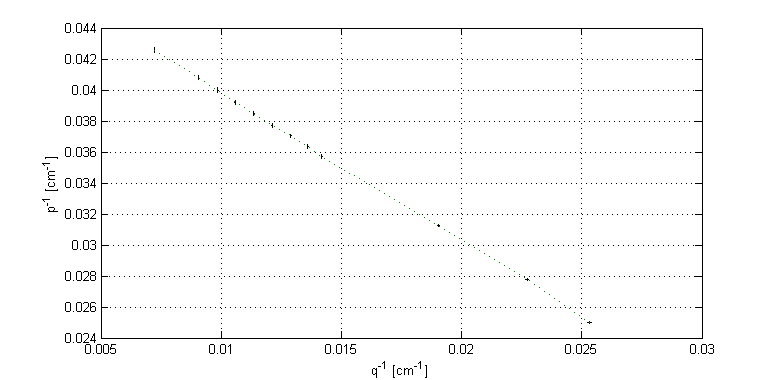
\includegraphics[scale=0.65]{graficoP_Q.png}


\end{figure}
\end{center}

Come ci aspettavamo dalla formula dei punti coniugati, la rappresentazione dei punti ha un andamento lineare. Ne segue che il parametro \textit{f} sarà il parametro b della retta $y=a\cdot x+b$, dove $y=q^{-1}$, $x=p^{-1}$. Ci aspettiamo inoltre che a=-1. Eseguendo il fit della funzione tramite regressione lineare abbiamo trovato i seguenti risultati:\\
\begin{center}

  
\begin{tabular}{|c|c|c|c|}
\hline $a \pm \delta a$ & $b \pm \delta b [cm^{-1}]$ & $\chi ^{2}\ped{sperimentale}$ & $\chi ^{2}\ped{teorico}$ \\ 
\hline -0.961 $\pm 0.004$ & 0.0495 $\pm 0.0001$ & 9.4 & 10 \\ 
\hline 
\end{tabular}
\end{center} 
Ci è quindi possibile ricavare il parametro $\textit{f}$ come $\frac{1}{b}$: $$\textit{f}=\frac{1}{b}=20.21 \pm 0.03\hspace{1 mm} cm$$

\section{Aberrazione cromatica e aberrazione sferica}
\subsection{Aberrazione cromatica}
In questa seconda parte dell'esperienza abbiamo cercato di valutare se la lente convergente in dotazione sia affetta da aberrazioni. Il primo tipo di aberrazione è l'aberrazione cromatica. Per verificarne la presenza, ci siamo serviti di due filtri colorati (uno rosso e l'altro blu) posti alternativamente davanti alla fonte luminosa. Abbiamo quindi misurato i parametri p e q relativi alle radiazioni passanti attraverso i due filtri colorati, così da verificare eventuali differenze. I risultati ottenuti sono:\\
\begin{center}
\begin{tabular}{|c|c|c|}
\hline $luce$ & $p [cm]$ & $q [cm]$ \\ 
\hline rossa & $37\pm 0.3$ & $44.5 \pm 0.5$ \\ 
\hline blu & $37\pm 0.3$ & $43 \pm 0.5$ \\ 
\hline 
\end{tabular}  
\end{center}
Notiamo subito che, tenendo il parametro p costante, q varia nei due casi presi un esame. Ciò significa che la nostra lente rifrange in maniera differente radiazioni luminose di lunghezza d'onda diversa. Ciò ha anche un'altra conseguenza. Prendiamo in esame la formula del costruttore di lenti: $$\frac{1}{\textit{f}}=(n-1)\cdot (\frac{1}{R \ped{1}}-\frac{1}{R \ped{2}})$$
dove n è l'indice di rifrazione, $R\ped{1}$ e $R\ped{2}$ sono i raggi di curvatura della lente. Se p e q variano al variare della lunghezza d'onda della radiazione luminosa rifratta, significa che n varia. Ne segue che $n=n(\lambda)$.
\subsection{Aberrazione sferica}
L'aberrazone sferica consiste nel diverso angolo di rifrazione delle radiazioni luminose dovuta alla curvatura della lente. Inseriamo a tale proposito una immagine esplicativa:
\begin{center} 
\begin{figure}[htpd]
\hspace{140 pt}
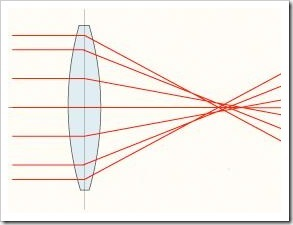
\includegraphics[scale=0.90]{aberrazione_sferica.png}


\end{figure}
\end{center}
Notiamo che dove la curvatura è maggiore, le radiaziioni vengono rifratte in maniera diversa rispetto al centro della lente, dove la curvatura è minore. Per misurare quantitativamente questo fenomeno ci siamo serviti di due diversi filtri da sovrappore alla lente, tra la lente e la fonte delle radiazioni. Il primo filtro lasciava passare solamente le radiazioni passanti per il centro della lente, dove la curvatura è minore. Il secondo filtro al contrario lasciava passare le radiazioni passanti per la parte periferica della lente, dove la curvatura è maggiore. Riportiamo quindi i parametri di p e q ottenuti:\\
\begin{center}
\begin{tabular}{|c|c|c|}
\hline $filtro$ & $p [cm]$ & $q [cm]$ \\ 
\hline 1 & $37 \pm 0.3$ & $44.5 \pm 0.5$ \\ 
\hline 2 & $37 \pm 0.3$ & $43.5 \pm 0.5$ \\ 
\hline 
\end{tabular} 
\end{center}
Notiamo che la lente presenta anche una aberrazione sferica.
\section{Calcolo dell'indice di rifrazione}
Per calcolare l'indice di rifrazione della lente ci rifacciamo nuovamente alla formula del costruttore di lenti. Tenendo conto della simmetria della lente, abbiamo: $$n=\frac{R}{2\textit{f}}+1$$
dove $textit{f}$ è la distanza focale precedentemente calcolata e R è il raggio di curvatura della lente. Servendoci del calibro ventesimale abbiamo calcolato R attraverso relazioni geometri elementari. Il valore di n trovato è: $$n = 1.56\pm 0.05$$
\end{document}